\documentclass[../main.tex]{subfiles}

\begin{document}
%%%%%%%%%%%%%%%%%%%%%%%%%%%%%%%%%%%%%%%%%%%%%%%%%%%%%%%%%%%%%%%%
%                                                              %
% Differentialrechnung III -- Differential, höhere Ableitungen %
%                                                              %
%%%%%%%%%%%%%%%%%%%%%%%%%%%%%%%%%%%%%%%%%%%%%%%%%%%%%%%%%%%%%%%%

\chapter{Differentialrechnung III -- Differential, höhere Ableitungen}

\section{Implizite Ableitung}
\textbf{Explizite Form}: $y = f(x)$ \\ [7pt]
Man kann für jedes x den Funktionswert berechnen und die Kurve zeichnen. \\ [7pt]
\textbf{Implizite Form}: $F(x,y) = 0$ \\ [7pt]
Oft ist eine Auflösung nach $y$ nicht möglich. \textbf{Leite Gliedweise nach $x$ ab, wobei $y = y(x)$ als Funktion von $x$ betrachtet werden muss und mit der Kettenregel ableiten.}

\subsection{Beispiel}
$x^2 + y^2 = R^2$ \\ [7pt]
$F(x,y) = x^2 + y^2 -R^2 = 0$ \\ [7pt]
$x^2 + (y(x))^2 -R^2 = 0$ $|$ differenzieren nach x, Achtung: Leite sowohl was links als auch rechts vom "=" ist!! \\ [7pt]
$2x + 2y(x) \times y'(x) -0 = 0$ \\ [7pt]
$y'(x) \times y(x) = -x$ \\ [7pt]
$y'(x) = -\frac{x}{y(x)} = -\frac{x}{\sqrt{R^2-x^2}}$

\subsection{y nach x}
\textbf{Kettenregel} \\ [7pt]
$y^3 = (y(x))^3$ \\ [7pt]
$3y(x)^2y'(x) = 3y^2y'$ \\ [14pt]
\textbf{Produkteregel Kettenregel} \\ [7pt]
$2xy^2 = 2x \times y^2$ $|$ Produkteregel!  \\ [7pt]
$(2x)' \times y^2 + 2x \times (y^2)'$ $|$ Kettenregel für $(y^2)'$\\ [7pt]
$(2x)' \times y^2 + 2x \times (2y^2 \times y')$ \\ [7pt]
$2y^2 + 2x \times 2yy' = 2y^2+4xyy'$

\section{Differential}
Um wieviel verändert sich die Funktion $y = f(x)$, wenn man sich von $x_0$ um $\Delta x$ entfernt? \\
Es gilt $\Delta y = f(x_0 + \Delta x) - f(x_0)$! \\
\begin{minipage}{0.5\textwidth}
    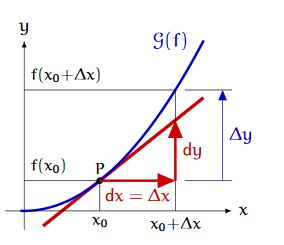
\includegraphics[width=50mm,scale=0.5]{differential}
\end{minipage} \hfill
\begin{minipage}{0.45\textwidth}
    Steigung der Tangente (blau) in $x_0$ \\ [7pt]
    $f'(x_0) = \frac{dy}{dx}$ \\ [7pt]
    Die Symbole $dx$ und $dy$ nennt man \textbf{Differentiale}. Das \textbf{Differential von $f$ an der Stelle $x_0$} ist \\ [7pt]
    $dy = f'(x_0)dx$ \\ [7pt]
    Es gilt also approximativ: \\ [7pt]
    $\Delta y \approx dy = f'(x_0)dx$
\end{minipage}
Statt $dy$ und $\Delta y$ verwendet man auch die Bezeichnung $df$ und $\Delta f$. \\

\begin{itemize}
    \item Das Differential $df = dy = f'(x)dx$ der Funktion $y = f(x)$ an der Stelle x ist gleich der Änderungen des Ordinaten- oder y-Wertes der Tangente durch $P(x,f(x))$, wenn man den Abszissen- oder x-Wert um $dx = \Delta x$ ändert.
    \item Das Differential $dy$ von $y = f(x)$ an der Stelle x wird verwendet, um die wahre Änderung von $\Delta y$ zu approximieren \\ [7pt]
    $\Delta y \approx dy = f'(x)dx$ \\ [7pt]
    Diese Approximation ist umso genauer, je kleiner $dx = \Delta x$ ist.
    \item Das Differential $dy$ ist gleich der Änderung der an der Stelle x linearisierten Funktion, wenn sich x um $dx = \Delta x$ ändert.
    \item Für eine lineare Funktion gilt somit $dy = \Delta y$
    \item Vorteil gegenüber der exakten Änderung: die Berechnung für ein anderes $dx = \Delta x$ ist lediglich eine Multiplikation mit $f'(x)$
\end{itemize}

\subsection{Beispiel Differential}
Sei $f(x) = x^2 + e^{x-1}$. Um wieviel verändert sich f, wenn x von 1 auf 1.1 erhöht wird? \\
$f(x) = x^2 + e^{x-1}$ \\
$x_0 = 1, x_1 = 1.1$ \\ [7pt]
\textbf{Exakt}: \\ [7pt]
$f(x_1) - f(x_0) = 1.1^2 + e^{1.1-1} - (1^2 + e^{1-1})= 1.21 + e^0.1 - 2 = 0.315$ \\ [7pt]
\textbf{Approximativ}: \\ [7pt]
$f'(x) = 2x + e^{x-1} \times 1$ \\ [7pt]
$f'(x_0) = 2 \times 1 + e^{1-1} = 3$ \\ [7pt]
$f'(x) = 3 = \frac{dy}{dx}; dy = 3dx$ $|$ Differentialschreibweise \\ [7pt]
$\Delta y = f(x_1) - f(x_0); \Delta x = x_1 - x_0$ \\ [7pt]
$\Delta y \approx dy = 3dx \approx \Delta x = 3 \times 0.1 = 0.3$

\subsection{Rechenregeln für Differentiale}
\begin{tabularx}{0.8\textwidth} { 
    >{\centering\arraybackslash}X 
    >{\centering\arraybackslash}X  }
    \hline
    Ableitungsregeln & Regeln für Differentiale \\ [7pt]
    \hline
    $[c]' = 0$ & $d[c] = 0$
    \\ [7pt]
    $[cf]' = cf'$ & $d[cf] = cdf$
    \\ [7pt]
    $[f + g]' = f' + g'$ & $d[f+g] = df +dg$
    \\ [7pt]
    $[fg]' = f'g + fg'$ & $d[fg] = df \times g +f \times dg$
    \\ [7pt]
    $[\frac{f}{g}]' = \frac{f'g - fg'}{g^2}$ & $d[\frac{f}{g}] = \frac{df \times g - f \times dg}{g^2}$
\end{tabularx}

\section{Monotonie}
\begin{itemize}
    \item Gilt $f'(x) > 0$ in einem Intervall I, dann ist f dort \textbf{streng monoton wachsend}.
    \item Gilt $f'(x) \geq 0$ in einem Intervall I, dann ist f dort \textbf{monoton wachsend}.
    \item Gilt $f'(x) < 0$ in einem Intervall I, dann ist f dort \textbf{streng monoton fallend}.
    \item Gilt $f'(x) \leq 0$ in einem Intervall I, dann ist f dort \textbf{monoton fallend}.
\end{itemize}

\subsection{Lokale oder relative Extrema}
Notwendige Bedingung für ein lokales Extremum von f in $x_0$:
$f'(x_0) = 0$ Diese Bedingung ist aber nicht hinreichend, es ist erst ein \textbf{kritischer Punkt} \\ [14pt]
Wenn $f'(x_0) = 0$ \textbf{und}: \\
$f''(x_0) > 0$ dann liegt ein lokales (oder relatives) Minimum vor.
$f''(x_0) < 0$ dann liegt ein lokales (oder relatives) Maximum vor.

\section{Höhere Ableitungen}
$y'' = f''(x) = \frac{d}{dx}[f'(x)] = \frac{d}{dx}(\frac{dy}{dx}) = \frac{d^2y}{dx^2}$ \\ [7pt]
\textbf{Geometrische Bedeutung:} die 2. Ableitung ist positiv wenn die 1. Ableitung (also die Steigung) zunimmt wenn man sich in Richtung zunehmender x entlang der Kurve bewegt.
\begin{itemize}
    \item Gilt $f''(x) > 0$ in einem Intervall I, dann weist f dort eine \textbf{Linkskrümmung} auf. Wir sagen f ist \textbf{konvex}.
    \item Gilt $f''(x) < 0$ in einem Intervall I, dann weist f dort eine \textbf{Rechtskrümmung} auf. Wir sagen f ist \textbf{konkav}.
\end{itemize}

\section{Krümmung}
Die Krümmung der Kurve $y = f(x)$ an der Stelle x ist: \\ [7pt]
$K(x) = \frac{y''(x)}{[1+(y'(x))^2]^{\frac{3}{2}}}$ ; Krümmungskreisradius $p(x)=\frac{1}{|K(x)|}$ \\ [7pt]
Für $K > 0$ hat man eine Links- und für $K < 0$ eine Rechtskrümmung.


\end{document}